\section{Transfer Learning}

\begin{figure*}
	\centering
	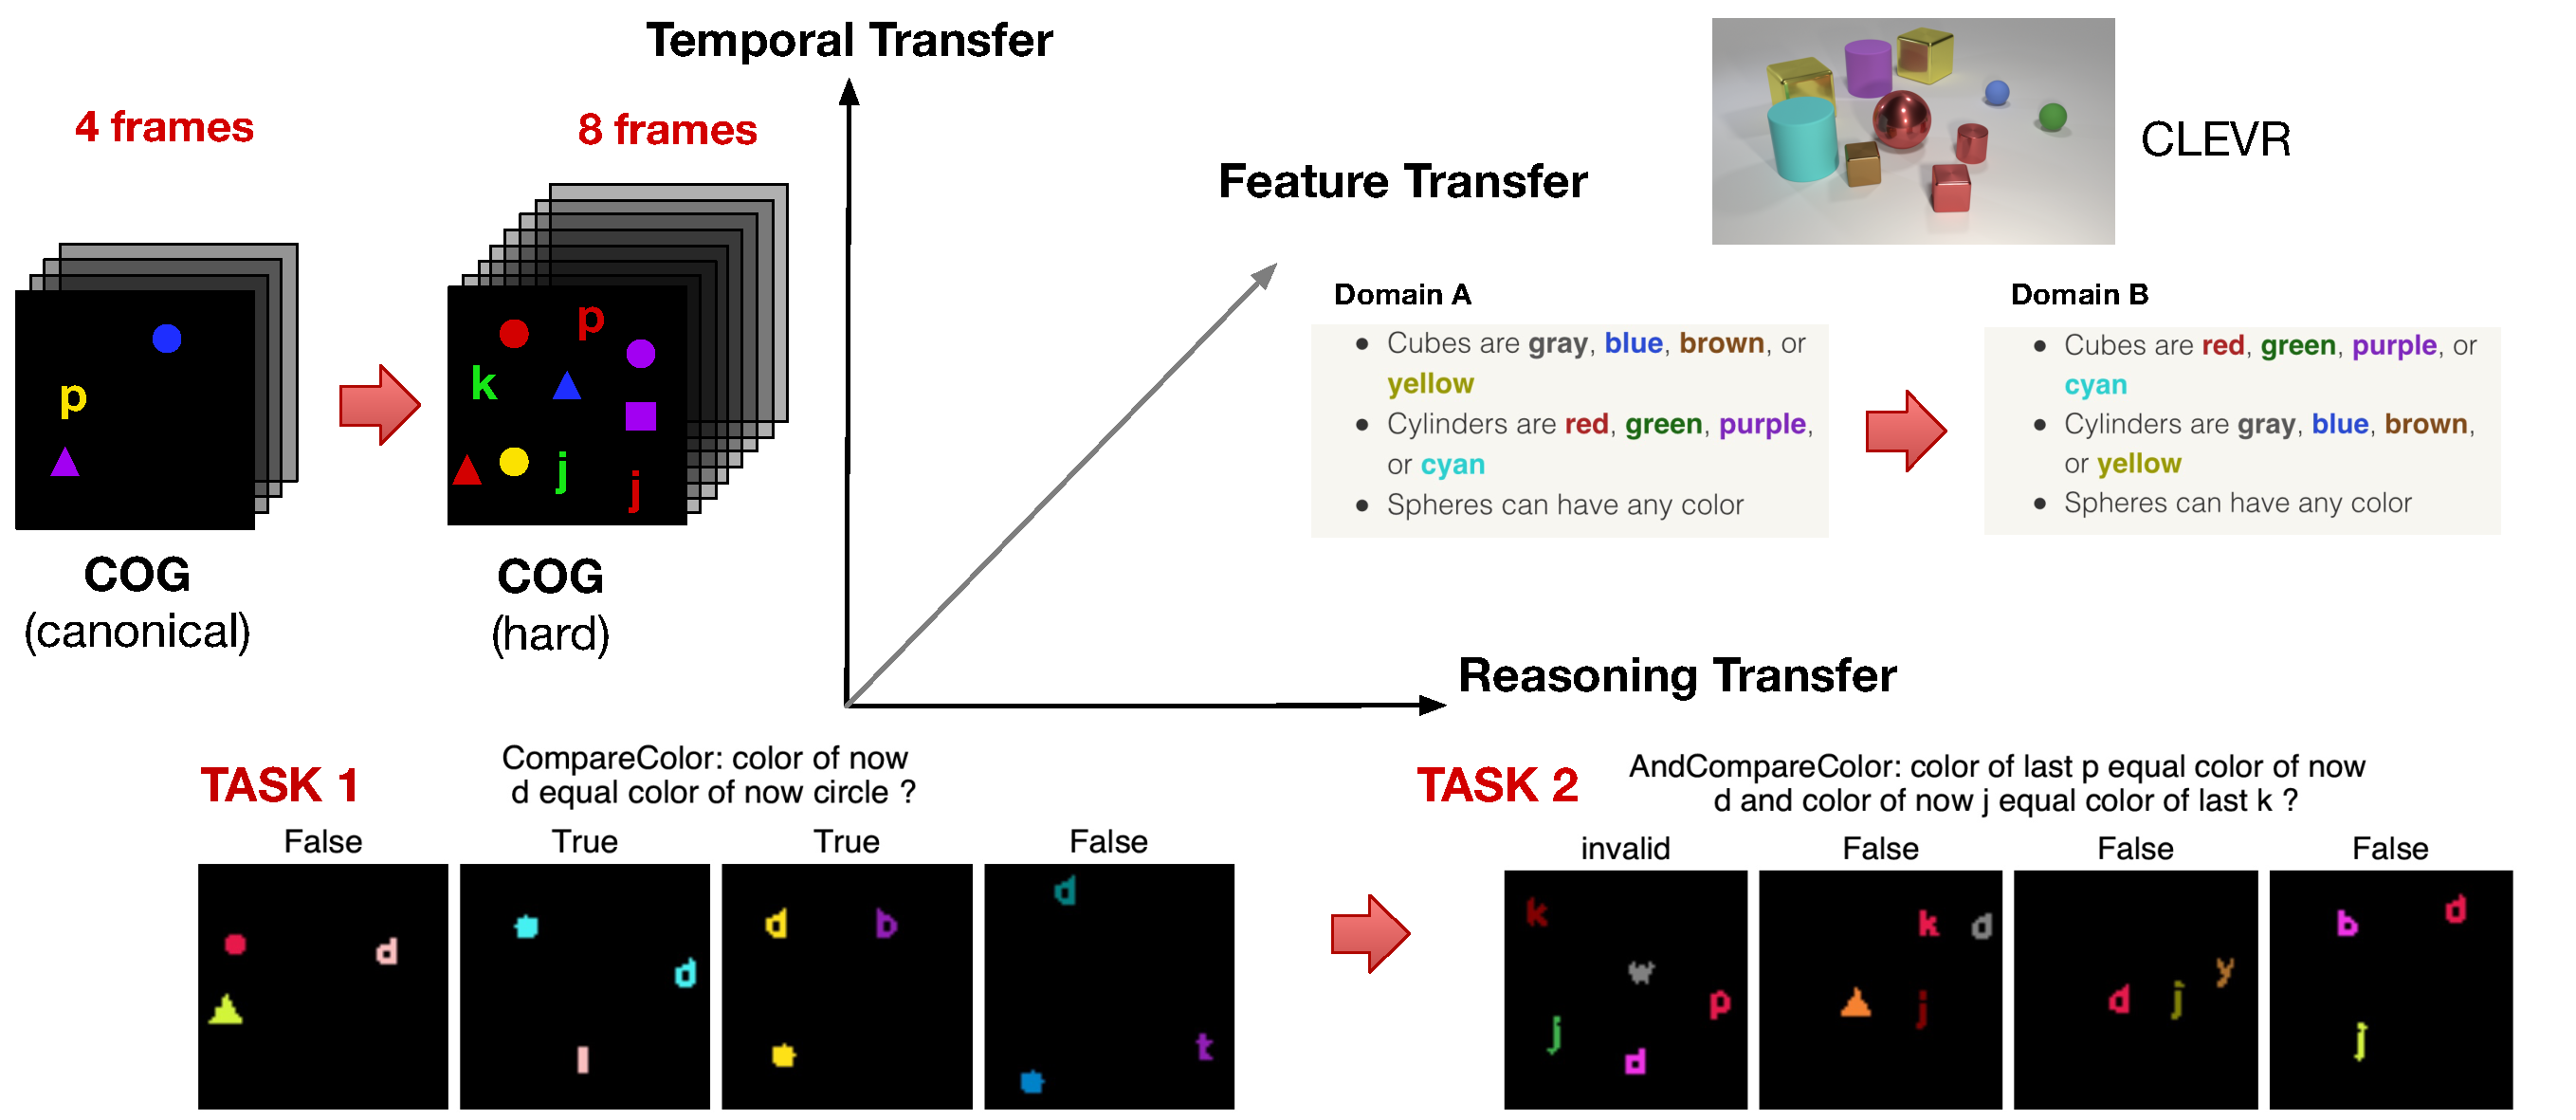
\includegraphics[width=0.9\textwidth]{../img/architecture/transfer_taxo}
	\caption{Transfer learning taxonomy.}\label{fig:taskonomy}
\end{figure*}
Due to the complex nature of visual reasoning, it appears that
transfer learning from a source domain to a target domain can be investigated in
multiple ways, depending on how the features are related between the two domains. This includes attributes such as size, color and shape, as well as temporal characteristics reflected in the number of frames and the scene complexity.
To establish a formal framework for these various aspects, we first recall the basic definition of transfer learning~\cite{pan2009survey}.

A \emph{domain} is a pair $\cD = (\cX,P(X))$, where $\cX$ is a feature space and $P(X)$ is a marginal probability distribution.
For visual reasoning problems considered in this paper,
$\cX$ will consist of purely visual inputs, i.e., either images or videos in some cases, or
a combination of both visual inputs and questions in other cases.
A \emph{task} is a pair $\cT= (\cY,f(\cdot))$, where $\cY$ is a label space and $f: \cX \to \cY$ is a prediction function.
When the domain elements consist of both the question and the visual input, there is only one task, namely, to answer the
question\footnote{%
	For the COG dataset, the answer is a tuple, one for each frame in the video, whereas for typical video answering datasets,
	only a single answer is needed for the entire video.}. %
If the domain elements consist of just the visual inputs, then the task is defined by the question so that each question
defines a separate task.

\begin{definition}[\cite{pan2009survey}]
	\label{defn:transfer}
	Given a source domain $\cD_S$ and a source learning task $\cT_S$, a target domain $\cD_T$ and a target learning task $\cT_T$, transfer learning aims to help improve the
	learning of the target predictive function $f_T(\cdot)$ in $\cD_T$ using the knowledge  in $\cD_S$ and $\cT_S$, where $\cD_S \ne \cD_T$, or $\cT_S \ne \cT_T$.
\end{definition}
In all our applications, $\cX_S = \cX_T$, so $\cD_S \ne \cD_T$ means that the marginal distributions $P_S$ and $P_T$ are different.
Similarly, $\cT_S \ne \cT_T$ means that either $Y_S \ne Y_T$ or that the associated prediction functions are different.

Although~\cref{defn:transfer} is quite general, it does not adequately capture all artifacts present in visual reasoning.
For example, consider the transfer learning setting where the tasks $\cT_S$ and $\cT_T$ are the same
but the marginal distributions $P_S$ and $P_T$ are different (referred to as \emph{domain adaptation}).
As mentioned in the introduction, one setting is the case of static images,
where this could be due to having different feature combinations in the source and target.
A different setting is in the context of video reasoning where the number of frames can increase significantly going from source to target.
These require possibly very different methods: the first involves building disentangled feature representations that can generalize across
domains; the second might need external memory to remember relevant objects to generalize across frame lengths.
Another situation is when the questions themselves can be grouped into families such as count-based queries,
comparison of objects, or existence of objects with certain features etc.
This entails studying transfer learning between families of tasks which requires extending the above definition.

We now formally define 3 kinds of transfer learning problems, namely,
\emph{feature transfer}, \emph{temporal transfer},
and \emph{reasoning transfer}.
These are illustrated in~\cref{fig:taskonomy} using representative examples from CLEVR-CoGenT and COG datasets that are particularly suited for experimental
investigations of transfer learning.
In the next section we detail the performance of
SAMNet for each of these 3 kinds, using the CLEVR-CoGenT dataset
for feature transfer, the COG dataset for temporal transfer, and finally
both datasets for reasoning transfer, with appropriate baseline comparisons.

Let $\cQ$ and $\cV$ denote the set of questions and visual inputs, respectively.
\begin{description}
	%\compresslist % used to reduce spacing
	\item[Feature Transfer:] In this setting of domain adaptation, $\cX_S = \cX_T \subseteq \cQ \times \cV$
	and the task $f(q,v)$ is just the answer to the question $q$ on visual input $v$. The output set $\cY$ is the union of legitimate answers
	over all questions in $\cQ$.
	The marginal distributions $P_S$ and $P_T$ differ in the feature attributes such as shape, color, and size, or their combinations
	thereof.

	\item[Temporal Transfer:] This setting is similar to attribute adaptation in that $\cX_S = \cX_T \subseteq \cQ \times \cV$
	and there is a single task.
	The key difference is that we introduce a notion of complexity $C(v) = (n, m)$ for a visual input $v$,
	where $n$ equals the maximum number of objects $n$ in an image, and $m$
	equals  the number of frames in a video.
	For any visual input $v_S$ coming from $\cX_S$ with $C(v_S) = (n_S, m_S)$
	and for any visual input $v_T$ coming from $\cX_T$ with $C(v_T) = (n_T, m_T)$, we require that $n_T \ge n_S$ and
	$m_T \ge m_S$ with at least one inequality being a strict one.
	Thus, we necessarily increase the complexity of the visual input going from the source to the target domain.

	\item[Reasoning Transfer:]
	This setting requires an extension of~\cref{defn:transfer} above to investigate transfer learning when
	grouping questions into families. Let $\cV$ be the feature space consisting of visual inputs only, shared by
	all tasks, with a common marginal distribution $P(X)$. For each question $q \in \cQ$, we define the task
	$\cT_q = (\cY_q, f_q(\cdot))$ where
	the output set $\cY_q$ is the set of legitimate answers to $q$ and $f_q(v)$, for a visual input $v$,
	is the answer to question $q$ on visual input $v$.
	Thus, tasks are in a 1-1 correspondence with questions.
	A \emph{task family} is a probability distribution on tasks which in our case can be obtained by defining the distribution on $\cQ$.
	Given a task family, the goal is to learn a prediction function that gives an answer to $f_q(v)$ for $v \in \cV$ chosen according
	to the feature space distribution and $q$ chosen according to the task probability distribution.
	Suppose $\cF_S$ is the source task family and $\cF_T$ is the target task family.
	Transfer learning aims to help improve the learning of the predictive function for the target task family
	using the knowledge in the source task family.

\end{description}

If labeled data is available for $\cX_T$, a training algorithm distinction we make is between \emph{zero-shot learning} and \emph{finetuning}. Finetuning entails the use of labeled data in the target domain $\cD_T$, foreseeing performance gain on the target task $\cX_T$, after initial training on $\cX_S$ and additional training on $\cX_T$. Zero-shot learning thus refers to immediate test on $\cX_T$ after initial training on $\cX_S$.
